\section{\large Introducción}
En Colombia, la gestión de fotocomparendos ha sido objeto de controversia debido a fallas en la transparencia y posibles manipulaciones en el proceso de registro y validación de infracciones. La falta de un sistema confiable ha generado desconfianza entre los ciudadanos, lo que evidencia la necesidad de una solución que garantice la integridad, inmutabilidad y verificabilidad de la información.

La tecnología Blockchain ha demostrado ser una alternativa eficaz para el almacenamiento seguro y descentralizado de datos, asegurando que una vez registrados, estos no puedan ser alterados sin dejar rastro. A través de contratos inteligentes, es posible automatizar la validación y el procesamiento de fotocomparendos, reduciendo la intervención humana y minimizando el riesgo de corrupción o errores administrativos.

Este trabajo propone el diseño e implementación de un prototipo basado en Blockchain para la gestión de fotocomparendos en Bogotá, con el objetivo de garantizar la transparencia del proceso. Se utilizarán contratos inteligentes para registrar cada infracción, permitiendo que cualquier actor autorizado pueda verificar su autenticidad sin necesidad de intermediarios. Mediante pruebas y simulaciones, se evaluará la viabilidad del sistema, demostrando cómo esta tecnología puede fortalecer la confianza en los procesos de control de tránsito y mejorar la eficiencia en la gestión de sanciones.

\subsection{Formulación del problema}
El sistema actual de gestión de fotocomparendos en Bogotá, enfrenta serias limitaciones en términos de transparencia, seguridad e integridad de la información, lo que genera desconfianza por parte de la ciudadanía y dificultades administrativas en su gestión. Según el Observatorio de Movilidad de Bogotá, entre enero de 2018 y agosto de 2024 se emitieron 5.575.982 comparendos, de los cuales el 48,91 \% fueron generados mediante dispositivos electrónicos de asistencia policial \parencite{ObservatorioComparendos2025}

\begin{figure}[htbp]
    \begin{flushleft}
        \textbf{Figura 1}\\[2em]
        \textit{Estadísticas de comparendos emitidos en Bogotá entre enero de 2018 y agosto de 2024}
    \end{flushleft}
    \vspace{1em}
    \addcontentsline{lof}{figure}{Figura 1. Estadísticas de comparendos emitidos en Bogotá entre enero de 2018 y agosto de 2024}
    \centering
    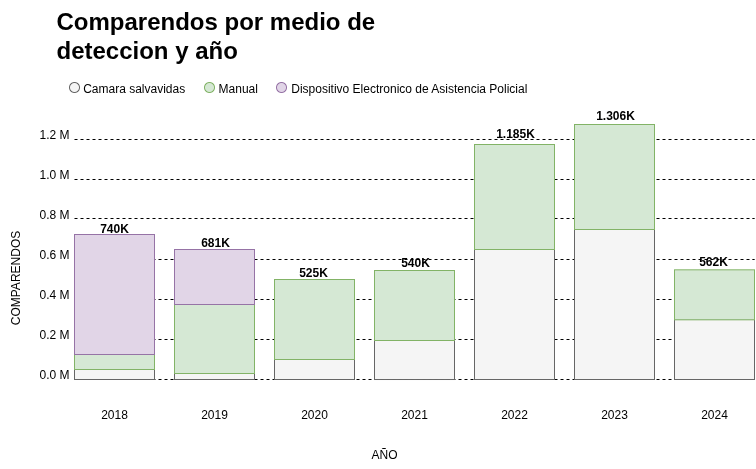
\includegraphics[width=0.8\textwidth]{Images/numComparendos.png}
    \vspace{2em}
    \begin{flushleft}
        \textit{Nota.} Elaboración propia con datos del Observatorio de Movilidad de Bogotá.
    \end{flushleft}
    \refstepcounter{figure}\label{fig:estadisticas_comparendos}
\end{figure}

Estas cifras reflejan el papel protagónico que tienen las fotomultas en la regulación del tránsito en la ciudad, pero también resaltan la necesidad urgente de fortalecer los mecanismos de manejo, almacenamiento y verificación de evidencias.  

La ausencia de un sistema confiable y auditable que permita garantizar la inmutabilidad de los registros, así como la trazabilidad de las evidencias, ha generado un entorno donde se cuestiona la validez de las sanciones, se incrementan las quejas ciudadanas y se limita la eficiencia operativa de las entidades encargadas del control de tránsito. En este contexto, surge la necesidad de explorar tecnologías emergentes, como Blockchain e IPFS, que podrían ofrecer una solución más segura, descentralizada y transparente para la gestión de estos procesos. 

\subsection{Objetivos}
\paragraph{Objetivo General}
Desarrollar un prototipo que gestione los fotocomparendos en Bogotá, utilizando tecnologías como Hyperledger Fabric e InterPlanetary File System, con el fin de lograr una gestión segura, auditable y descentralizada del proceso. 

\paragraph{Objetivos específicos}
\begin{itemize}
    \item Analizar el proceso actual de gestión de fotocomparendos en Bogotá, mediante la revisión de la normativa y una auditoría del sistema Fénix —el sistema que actualmente gestiona los fotocomparendos en Bogotá— para identificar las vulnerabilidades y los requisitos funcionales y no funcionales (seguridad, rendimiento y auditabilidad) que el prototipo debe satisfacer, resultando en una lista de requerimientos específicos para la nueva solución.
    \item Construir el prototipo del sistema de gestión de fotocomparendos, implementando la arquitectura propuesta (InterPlanetary File System para el almacenamiento de imágenes y Hyperledger Fabric para el registro de transacciones), asegurando que cada transacción contenga el hash único de InterPlanetary File System y los metadatos esenciales del comparendo (fecha, hora, lugar, placa, tipo de infracción), y desarrollando una interfaz básica que permita la carga de la evidencia y la consulta/verificación de los registros en la blockchain y la imagen en InterPlanetary File System, con el fin de materializar técnicamente la solución propuesta basada en los requisitos identificados en el objetivo anterior.
    \item Evaluar la efectividad y viabilidad del prototipo desarrollado, mediante la ejecución de un plan de pruebas funcionales (verificar la correcta carga a InterPlanetary File System, el registro inmutable en el ledger, la consistencia de datos, la capacidad de verificación) y pruebas de rendimiento básicas (medir tiempos de registro y consulta) en un entorno de simulación controlado, para validar que el prototipo cumple con los requisitos clave de inmutabilidad, transparencia y seguridad.
\end{itemize} 